\begin{highlightblock}[Pulse Width Modulation]

\begin{center}
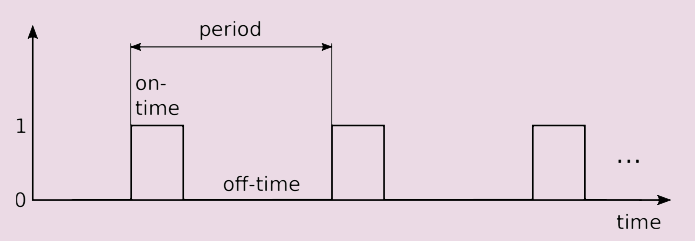
\includegraphics[width=0.7\linewidth]{images/PWM.png}

Figure \refstepcounter{figure}\arabic{figure}: Pulse Width Modulation\label{fig:pwm}
\end{center}
\vspace{-12pt}
In this exercise, a pulse width modulation (PWM) generator should be implemented.
An example PWM signal is schematically shown in Figure \ref{fig:pwm}. There the two
important parameters period (time) and on time is shown. These two parameters define
the so-called duty cylce: on time divided by period. The PWM generator will be used
for two tasks in this course: to control a servo motor and to build a digital to analog
converter (DAC). For these applications (more details will follow in later exercises),
the output level (either voltage or position of the servo) is defined via the duty cycle.
Use the following entity for the top-level design:

\lstinputlisting[
    caption={PWM entity},
    label={lst:pwm-entity},
    firstline=14,
    numbers=none
]{../pwm_e.vhd}

Why do you think the counter values for the period and the one-time are
specified as inputs?
\end{highlightblock}

\begin{highlightblock}[To-Do List]
\begin{itemize}
\item Draw a block diagram of the architecture of the PWM. Do you need to
have a finite state machine? If you do, please write a state diagram.
\item Write the entities and architectures that are required in VHDL. Use one
.vhd file for each entity and one .vhd file for each architecture.
\item Write a testbench in VHDL (extra file). Simulate the system using Modelsim
and hand in screenshots showing the output of the waveform window. Find meaningful
test cases. Please also include the test cases with a duty cycle of 0\% (the output
signal has to stay at 0 over the periods for this test case) and a duty cycle of
100\% (the output signal has to stay at 1 over the periods for this test case).
\item Discuss the results of the simulation in a few sentences and answer the
questions.
\end{itemize}
\end{highlightblock}